\setauthor{Abdulrahman Al Sabagh}
\begin{spacing}{1}


    \section{Probleme mit localhost und https}\label{sec:probleme-mit-localhost-und-https}

    Im Projekt wurde  die \textbf{U}niform \textbf{R}esource
    \textbf{L}ocater (URL) für den (API)-Server in einem ''.env-File'' gespeichert.
    Für die lokale Entwicklung wurde Strapi auf dem lokalen Host immer verwendet.
    Bei IOS und Android ist das Holen der Daten von nicht sicheren Quellen
    beziehungsweise nur von HTTP gar nicht möglich. Auf Android gibt aber einige
    Ausnahmen für das Holen der Daten von einem lokalen Host
    Bei Android kann man bei den generierten Build und Project Files einige Konfigurationen ändern.
    Das ist jedoch keine gute Lösung, da diese Files bei jedem Build geändert werden können.
    Außerdem können diese generierten Files nicht in das \textbf{V}ersion \textbf{C}ontrol \textbf{S}ystem (VCS)
    eingecheckt werden.
    Bei Android muss man die Adresse 10.0.2.2 statt localhost verwenden.\cite{androidFetch}
    Bei IOS gibt es keine einzige Möglichkeit,
    um Daten aus HTTP-Quellen oder aus dem localhost zu holen.
    Als Lösung wurde in der lokalen Entwicklung eine \textbf{C}ommand \textbf{L}ine \textbf{I}nterface (CLI) namens "ngrok" verwendet,
    welche den lokalen Port des Servers in das Internet mittels eines Tunnels weiterleitet
    und eine HTTPS-Adresse für den weitergeleiteten Server generiert. Somit schaut die Verbindung zwischen Client und Server wie folgendes aus:
    \begin{figure}[H]
        \centering
        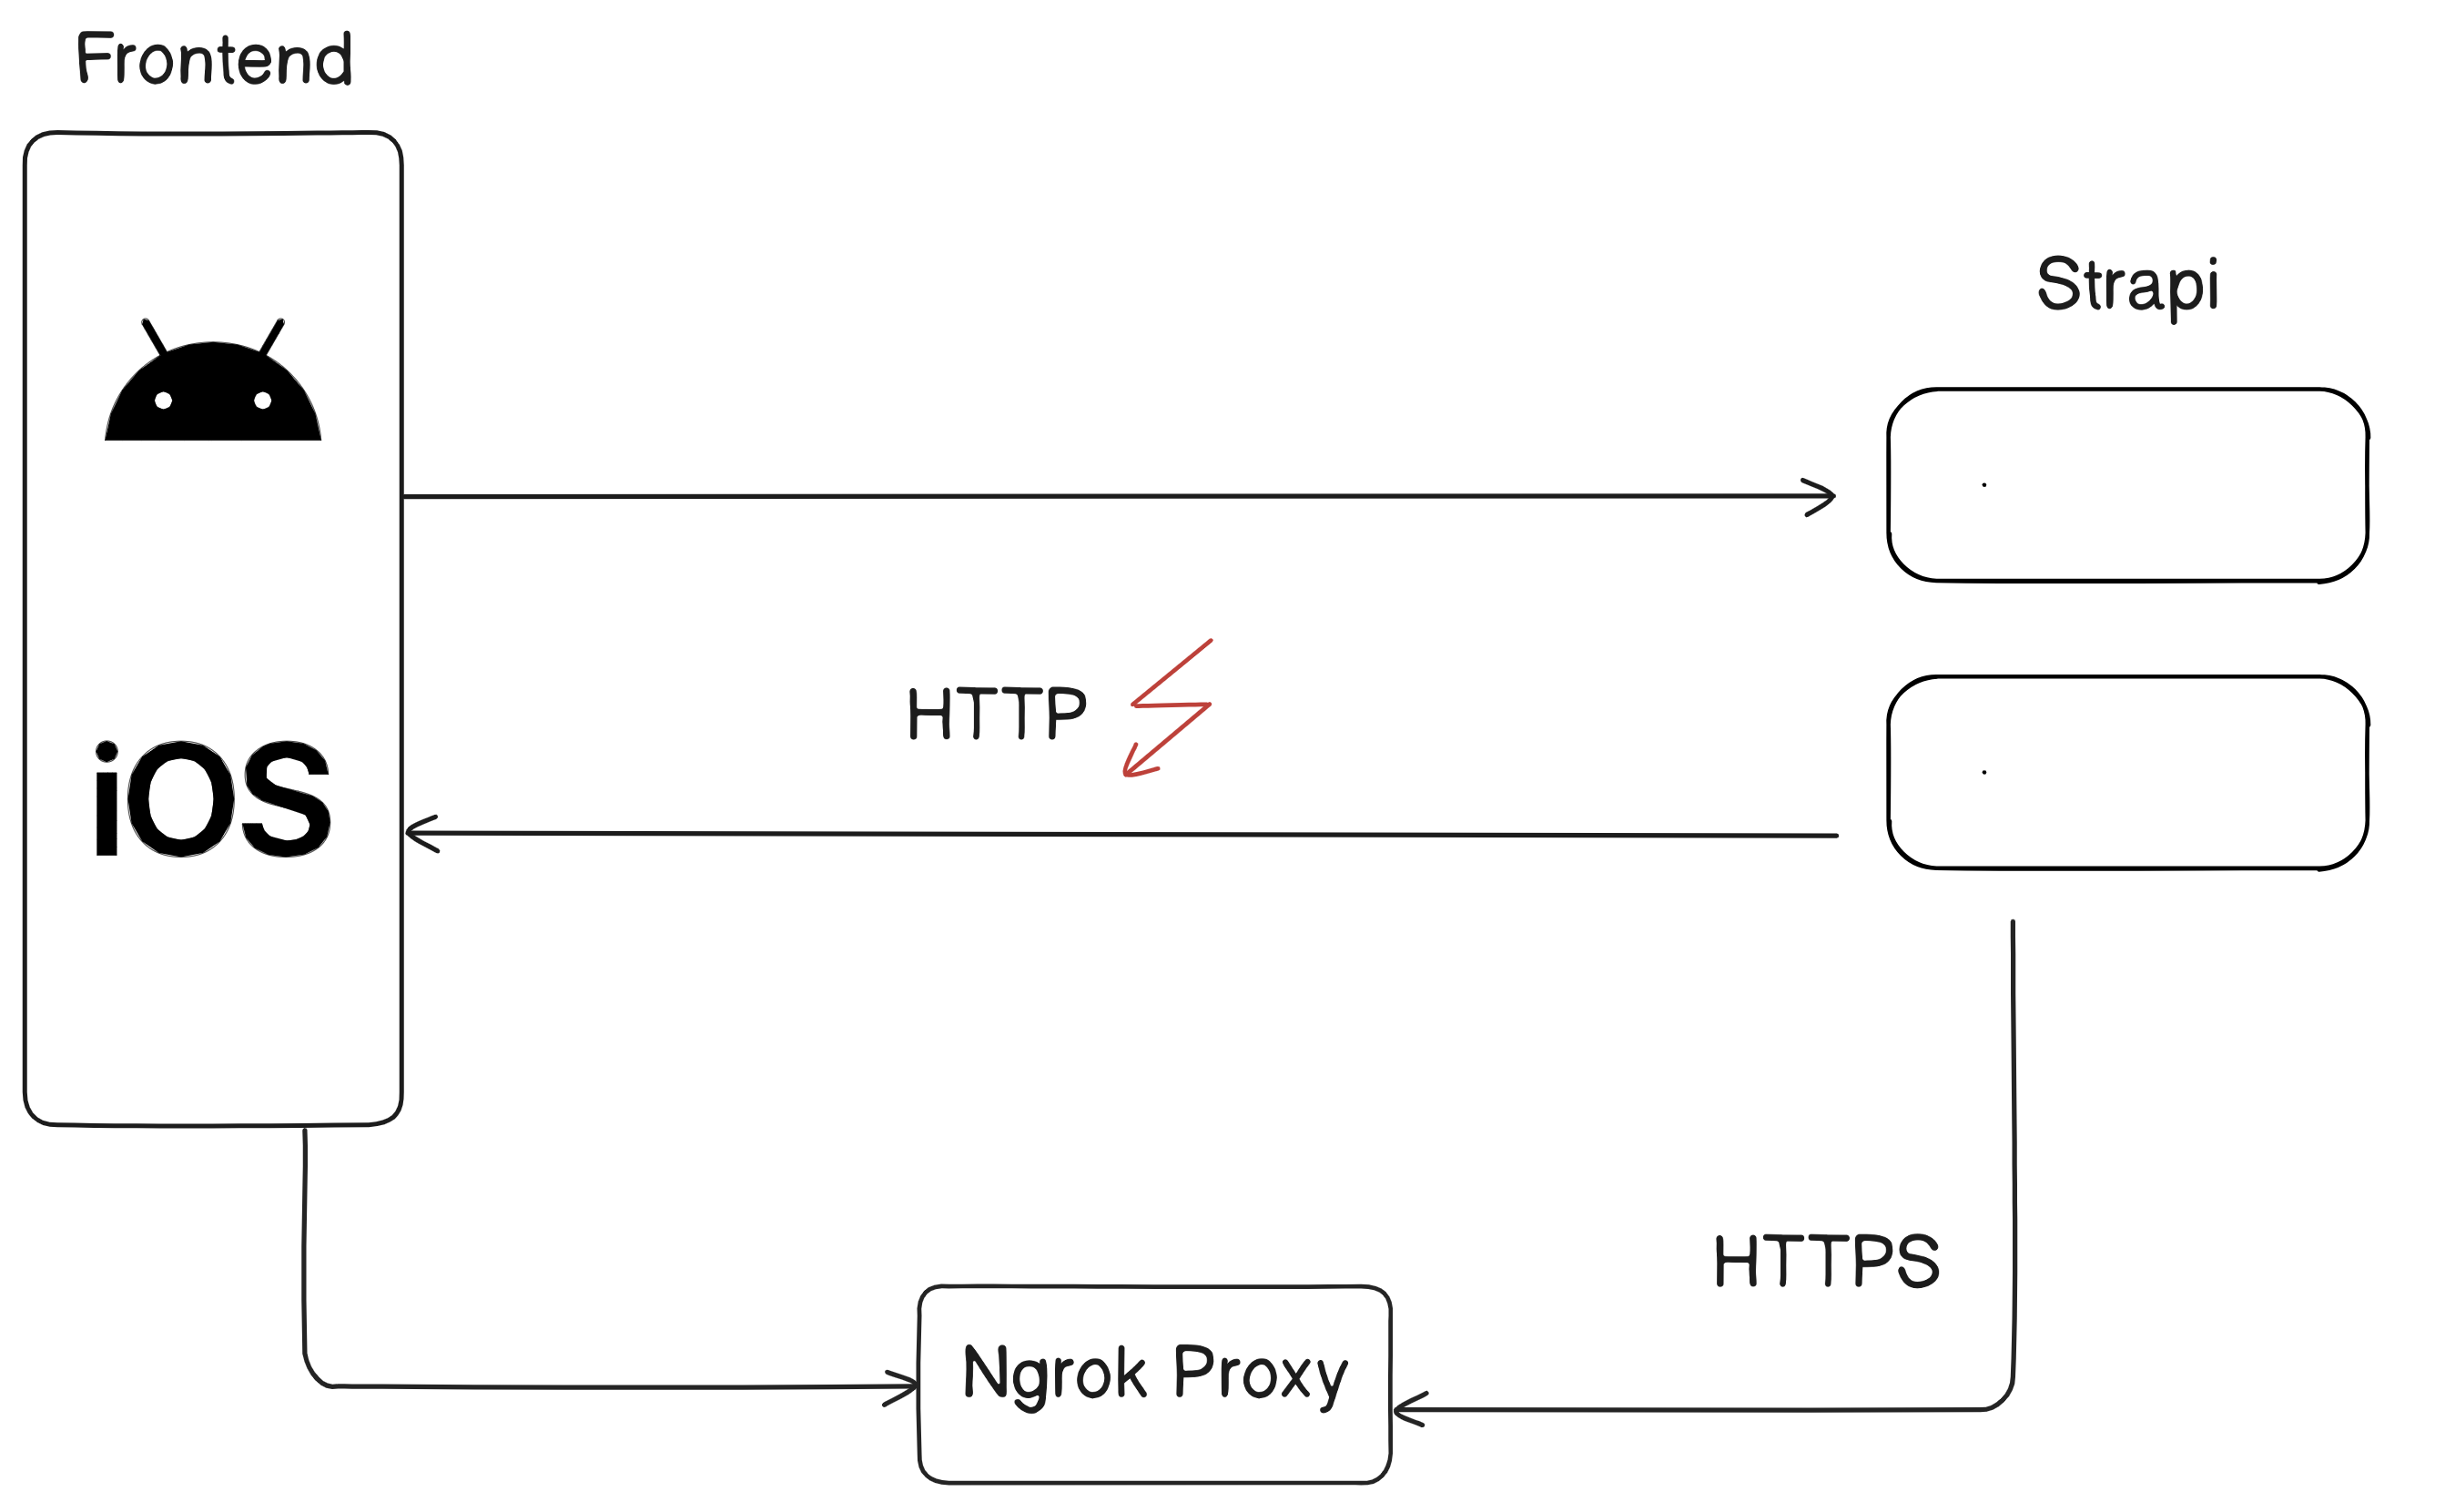
\includegraphics[width=\textwidth]{./pics/https-dev}
        \caption{ngrok}
    \end{figure}

    Das Problem tauchte wiederholt in der Testphase auf. Als Lösung hat sich das Team dieses mal ein Zertifkat besorgt. Nach dem Einbauen dieses Zertifkates hat sich die Verbindung zwischen Client und Server um einiges verändert. Diese schaut in dem produktiven System wie folgendes aus:
    \begin{figure}[H]
        \centering
        \includegraphics*[width=\textwidth]{./pics/https.png}
        \caption{HTTPS in prod}
    \end{figure}




    \section{Inkompatible Libraries beim Build-Prozess}\label{sec:inkompatible-libraries-beim-build-prozess}
    In der Entwicklungsphase wurden einige Libraries mittels \textbf{N}ode  \textbf{P}ackage \textbf{M}anager (npm) installiert.
    Einige Libraries waren mit der Node Version oder mit anderen Libraries nicht kompatibel.
    Eine Lösung wäre, das Label ''--legacy-peer-deps'' oder ''--force'' beim Befehl ''npm install'' anzuhängen.
    Während der Entwicklung wurde das Label ''--legacy-peer-deps'' immer beim ''npm install'' integriert
    und danach hat alles problemlos funktioniert.
    Später beim Deployment von Android ist das Problem
    bei der Generierung von Android apk bzw.
    \textbf{A}ndroid \textbf{A}pp \textbf{B}undle (aab) aufgetaucht.
    Die Apk bzw.
    Aab wurde erfolgreich generiert, aber die App war nicht funktionsfähig.
    Es wurde für das Finden des Problems auf Android ein Tool namens ''logcat'' verwendet,
    um die Fehlermeldung zu finden.
    Dieses Problem an sich ist in der Community sehr stark verbreitet und es gibt dafür mehrere Gründe und mehrere Lösungen.
    Unter diesem Githublink \cite{libjsexecutor} werden unterschiedliche Gründe und mehrere
    Lösungsmöglichkeiten für das Problem beschrieben.
    Es wurde jede einzelne Lösungsmöglichkeit versucht und keine von diesen vorgeschlagenen Lösungen
    funktionierte.
    Aus Erfahrung hat man gewusst, dass der Codebase einige Libraries besitzt,
    die nicht mehr gebraucht bzw.
    nicht mehr verwendet werden. Beim Löschen dieser Libraries und der Wiederinstallation
    von den Modulen mittels ''npm install'' tauchte die ''legacy-peer-deps'' Meldung wieder auf.
    Zur Problemlösung wurde ein Tool namens ''depcheck'' installiert,
    welches den Codebase scannt und dem Entwickler bekannt gibt, ob eine Library im Codebase verwendet
    wird oder nicht. \cite{depcheck}
    Nach dem Löschen aller nicht benötigten Libraries und die Generierung der
    Apk bzw.
    AaB hat die Applikation problemlos funktioniert.



    \subsection{npm install --legacy-peer-deps}\label{subsec:npm-install---legacy-peer-deps}
    \begin{quotation}
        ``
        The '--legacy-peer-deps' flag is used when you encounter compatibility issues with peer dependencies
        while installing packages.
        Peer dependencies are required by a package but aren't automatically
        installed alongside it.
        In some cases, when a package has not been updated to support the latest
        version of its peer dependency, the installation may fail due to conflicting versions.
        Adding the '--legacy-peer-deps' flag allows npm to use an older, compatible version of
        the peer dependency, ensuring a successful installation.''
        \cite{installFlags}
    \end{quotation}

    \subsection{npm install --force}\label{subsec:npm-install---force}
    \begin{quotation}
        ``
        The '--force'  flag is a more drastic option and should be used with caution.
        It instructs npm to forcefully install packages, even if it encounters errors or conflicts.
        This can be useful in situations where you want to override any version or compatibility checks
        and forcibly install packages.
        However, it is important to note that using '--force'
        may lead to unexpected issues, such as breaking dependencies or introducing incompatibilities,
        so it should be used sparingly and with a good understanding of its consequences.''
        ~\cite{installFlags}
    \end{quotation}



    \section{Probleme mit Thumbnails}\label{sec:probleme-mit-thumbnails}


    Relaxoon zeigt mehrere Videos für Antistress-Meditationen an. Damit diese schön darstellbar sind,
    muss jedes Video unbedingt ein Thumbnail haben.
    Der Content-Manager könnte aber beim Erstellen des Videos vergessen,
    ein Thumbnail für das Video zu erstellen.
    Auf der Adminoberfläche können keine Thumbnails zu dem Video hinzugefügt werden,
    da diese Aktion sehr schlechte User Experience verursacht.
    Man kann zwar eine Funktion implementieren,
    die nach dem Hochladen eines Videos ein Thumbnail mittels \textbf{F}ast \textbf{F}orward \textbf{M}oving
    \textbf{P}icture \textbf{E}xperts \textbf{G}roup (ffmpeg) aus dem ersten Bild des Videos erstellt.
    Diese Möglichkeit ist aber sehr aufwendig und nicht empfehlenswert, da die damalige Dokumentation von
    Strapi nicht sehr genau war.
    Außerdem könnte diese Alternative bei den Updates von Dependencies nicht mehr funktionsfähig sein.
    Darauf wurde eine Expo-Library gefunden, die im Frontend Thumbnails für die Videos erstellt.
    Die Verwendung davon war aber nicht sehr vorteilhaft, da der Generierungsprozess sehr langsam war.
    Als Lösung wurde im Code ein nicht abspielbares Videoelement deklariert,
    dass für den Zuschauer als Thumbnail dient.
    Das Video ist erst abspielbar, wenn man darauf klickt.
    Diese Lösung wurde mit den Konzepten ''Lazy Loading'' und ''Suspenses'' zusammen kombiniert,
    damit Loading-Spinners statt leere Flächen für den User angezeigt werden,
    wenn das Laden des Videos etwas länger dauert.



    \subsection{Suspense}\label{subsec:suspense}

    \begin{quotation}

        ``<Suspense> lets you display a fallback until its children have finished
        loading.''~\cite{suspense}
    \end{quotation}

    \subsection{Lazy Loading}\label{subsec:lazy-loading}

    \begin{quotation}
        ``lazy lets you defer loading component’s code until it is rendered for
        the first time.''~\cite{lazyLoading}
    \end{quotation}


    \section{Dauer von Videos}\label{sec:dauer-von-videos}

    Beim Hochladen eines Videos in Strapi
    wird die Dauer des Videos nur auf der Oberfläche angezeigt.
    Diese Information ist aber in den REST-Schnittstellen der Meta-Daten von den Files nicht inkludiert.
    Bei diesem Problem ist die Verwendung von ffmpeg auch eine Lösungsmöglichkeit.
    Es wurde aber nicht mit ffmpeg gearbeitet (siehe obiges Problem).
    Für die Berechnung der Dauer wurde im Frontend das "onLoad" Event,
    welches in den Properties (props) des Videoelements ist, verwendet,
    um die Dauer zu lesen und diese in das Format "mm:ss" umwandeln zu können.





    \section{Probleme mit useEffect und React-navigation Library}\label{sec:probleme-mit-useeffect-und-react-navigation-library}
    Für das Holen der Daten aus dem Server wurde die Fetch API verwendet.
    Diese wurde auch in einem ''useEffect Hook'' eingegeben, damit die Daten bei jeder Aktualisierung eines spezifischen
    Zustandes aus dem Server geholt werden können.
    Beim Anklicken der unterschiedlichen Navigationsbuttons wurde bemerkt,
    dass die Daten sich gar nicht ändern.
    Am Anfang wurde vermutet, dass das Problem ein Caching Problem sein könnte.
    Später wurde herausgefunden, dass die Library ''React-navigation'' den ''useEffect Hook'' im Hintergrund deaktiviert.
    Für das Holen der Daten ist die Übergabe eines sogenannten
    ''useCallback Hooks'' als Parameter in einem custom hook namens ''useFocusEffect''
    von React-navigation notwendig.\cite{issuesWithUseEffect}


    \subsection{Hooks}\label{subsec:hooks}
    \begin{quotation}
        ``Hooks let you use different React features from your components.
        You can either use the built-in Hooks or combine them to build your own.
        This page lists all built-in Hooks in React.''
        \cite{hooks}
    \end{quotation}

    \subsection{useEffect}\label{subsec:useeffect}
    \begin{quotation}
        ``useEffect is a React Hook that lets you synchronize a component
        with an external system.''~\cite{useEffect}

    \end{quotation}
    \begin{quotation}
        ``Some components need to synchronize with external systems.
        For example, you might want to control a non-React component based on the React state, set up a server connection,
        or send an analytics log when a component appears on the screen.
        Effects let you run some code after rendering so that you can synchronize your component with some system outside of React.[...]
        Effects let you specify side effects that are caused by rendering itself,
        rather than by a particular event. ''
        \cite{Synchronizing-with-effects}


    \end{quotation}


    \subsection{useCallback}\label{subsec:usecallback}
    \begin{quotation}
        ``useCallback is a React Hook that lets you cache a function definition between re-renders.''
        \cite{useCallback}
    \end{quotation}


    \subsection{useFocusEffect}\label{subsec:usefocuseffect}
    \begin{quotation}
        ``The useFocusEffect is analogous to React's useEffect hook. The only difference is that it only runs if the screen
        is currently focused.
        The effect will run whenever the dependencies passed to React.useCallback change,
        i.e. it'll run on initial render (if the screen is focused) as well as on subsequent renders if the dependencies
        have changed. If you don't wrap your effect in React.useCallback, the effect will run every render if the screen
        is focused.'' \cite{useFocusEffect}

    \end{quotation}

    \section{Probleme mit Dependency Updates}

    Im Laufe der Implementierungsphase wurden einige Dependencies wie React Native oder Strapi ein oder zweimal upgedatet. Bei einige Libraries haben die Updates problemlos funktioniert. Bei anderen wie zum Beispiel ''Expo Cli'' war es so, dass das Program nach dem Update nicht mehr lauffähig war. Daher hat man sehr viele Einstellungen in dem Program ändern müssen, damit das Program funktionieren kann.
    Bei der Library ''JWT-Decode'', welche wir für die Dekodierung von dem JWT verwendet haben, hat der Code am Beginn problemlos funktioniert. Nach einem Update kam es dazu, dass die Library den Token gar nicht deocdieren konnte.
    Nach einer langen Recherche kam man darauf, dass man ab der vierten Version eine Library namens ''base-64'' installieren soll.
    Danach soll diese importiert werden und als ein Singleton in dem Projekt definiert werden.
    \begin{lstlisting}[caption=base-64 als Singleton]
    import { decode } from 'base-64';
    global.atob = decode;
    \end{lstlisting}
    \begin{quotation}
        \cite{jwt-decode-bug}

    \end{quotation}
    Ein anderes Beispiel, wo das gleiche Problem wieder auftauchte, war bei der Aktualisierung von der Library ''Native base''. Es wurde herausgestellt,
    dass die vor dem Update verwendete Version von Native Base ist die letzte, die vom Hersteller unterstützt wird.

    \section{Relaxoon Plakat}\label{sec:plakat}
    \setauthor{Moritz Eder}

    Im Zuge des Projektes wurde mithilfe von Adobe Illustrator ein Plakat zur Repräsentation der mobilen App
    entwickelt.

    \section{Probleme mit dem Datenmodell}
    Nach der Realisierung wurde herausgestellt, dass das ERD doch um einiges verbessert werden kann. In dem folgenden Bild ist das neue Design von dem verbesserten ERD zu finden.
    \begin{figure}[H]
        \centering
        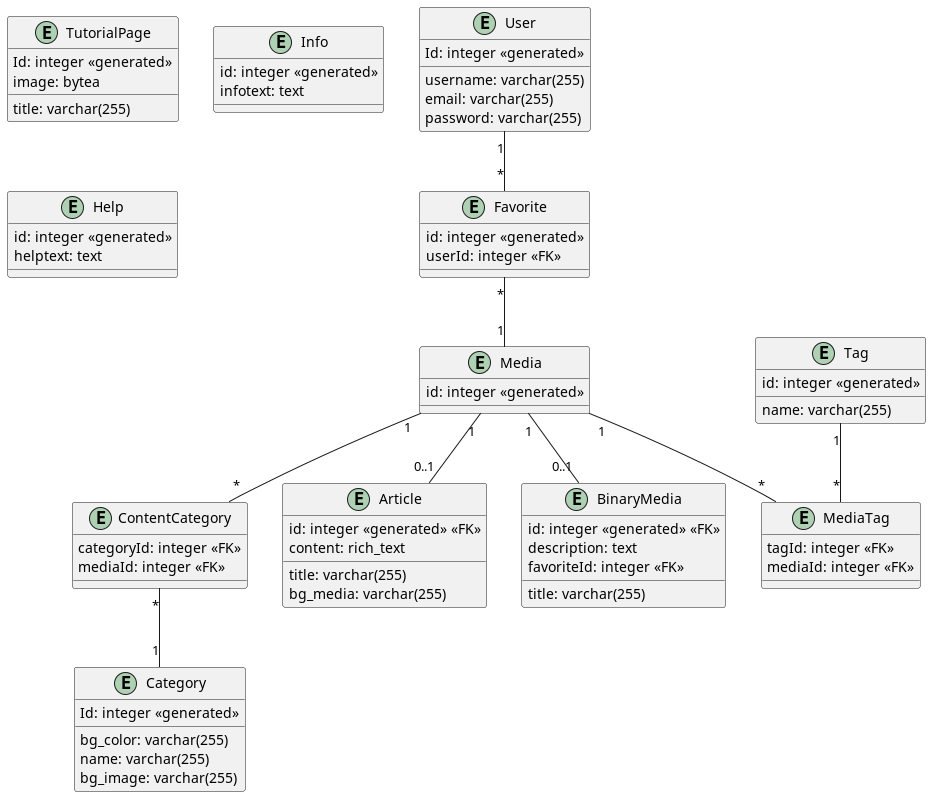
\includegraphics[width=\textwidth]{./pics/new-erd}
        \caption{new erd}
    \end{figure}

    Die Vorteile dieser Verbesserungen liegen dabei, dass man alle Arten von Medien nur mit einer einzigen SQL-Query abfragen kann. Außerdem ist die Komplexität um einiges reduziert, da nicht jede Medienart eine Beziehung zu den Tags und Kategorien hat.
    Vorher waren zwei Queries nötig, um alle Arten der Medien abzufragen.

    \subsection{Umsetzungsschritte}

    \begin{enumerate}
        \item Ein Farbverlauf wurde bestimmt, der sich von der hellblauen Farbe \#64C5DF (Hexadezimalschreibweise)
              bis zu einem dunkleren Blau \#3A62AC streckt. Der Farbverlauf dient als eine Grundlage des Plakates.
        \item Abgerundete Dreiecke sowie die abstrakte Form, welche am Rand des Plakats entlang geht,
              wurden in Kombination mit dem Farbverlauf erzeugt und platziert.
        \item Die Logos von Relaxoon, der HTL Leonding, den Firmen Solvistas und Macolution, dem CMS Strapi und der Programmiersprache React Native wurden hinzugefügt.
        \item Der Diplomarbeitsbetreuer und die Projektpartner wurden namentlich erwähnt.
        \item Das Grundlayout eines Smartphones wurde erstellt und mit einem Entwurf des Tutorials der App versehen.
        \item Fotos und Namen der App-Entwickler wurden eingefügt.
        \item Mit einem kurzen Beschreibungstext wurde das Plakat fertiggestellt.
    \end{enumerate}


    \begin{figure}[H]
        \centering
        
\includegraphics[height=1.4\textwidth]{./pics/Relaxoon-Plakat.jpg}
        \caption{Plakat}
    \end{figure}


\end{spacing}
\setauthor{Moritz Eder}


